\chapter{Projekt i implementacja aplikacji klienckiej}

\section{Funkcje aplikacji - diagram przypadków użycia}

Użytkownik:
\begin{itemize}
	\item tworzenie nowego konta (podanie loginu, hasła itp.);
	\item logowanie;
	\item przeglądanie filmów, seansów, kupionych biletów;
	\item kupowanie biletów.
\end{itemize}
\vspace*{0.5em}
Administrator:
\begin{itemize}
	\item te same funkcjonalności co użytkownik;
	\item dodawanie/usuwanie/edytowanie seansów;
	\item dodawanie/usuwanie/edytowanie filmów;
	\item dodawanie/usuwanie/edytowanie dostępnych sal.
\end{itemize}

\begin{figure} [H]
	\centering
	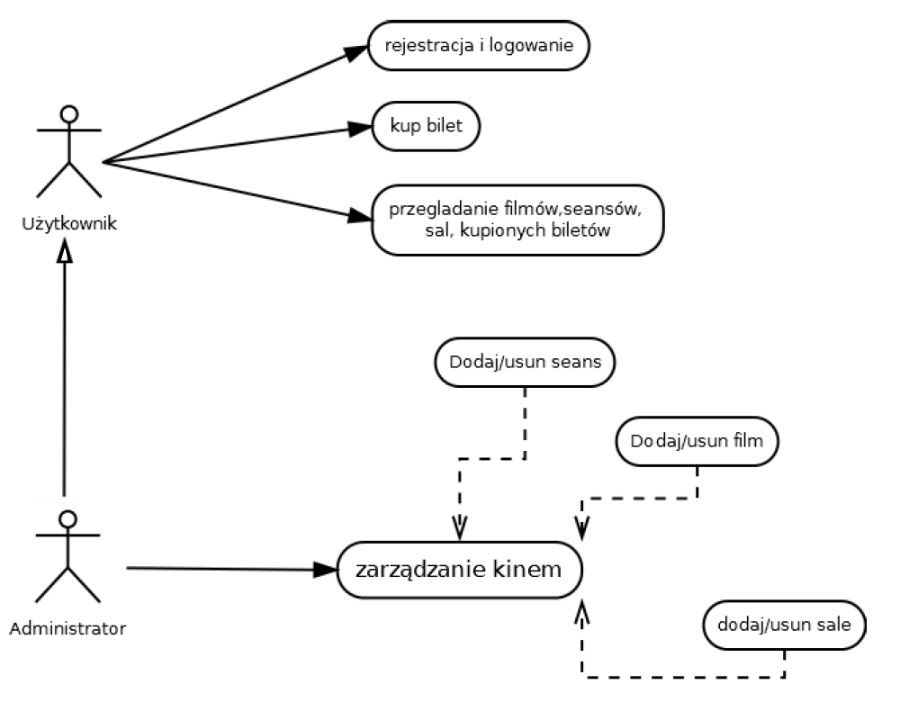
\includegraphics[width=0.6\linewidth]{rozdzial05/diagram.png}
	\caption{Diagram przypadków użycia}
	\label{fig:schem}
\end{figure}

\section{Realizacja wybranych funkcjonalności}